\subsection{LEAST UPPER BOUND AND GREATEST LOWER BOUND}

DEFINITION 6. Let E be an ordered set and let X be a subset of E. An element of E is said to be the greatest lower bound or infimum (resp. least upper bound or supremum) of X in E if it is the greatest (resp. least) element of the set of lower (resp. upper) bounds of X in E.

Given a subset X of an ordered set E, the least upper bound (resp. greatest lower bound) of X in E, when it exists, is denoted by

\[
\sup _ {\mathbf {E}} \mathbf {X} (\text { resp.   inf } _ {\mathbf {E}} \mathbf {X})
\]

or by sup X (resp. inf X) if there is no risk of ambiguity. The least upper bound (resp. greatest lower bound) of a set \(\{x, y\}\) of two elements, when it exists, is denoted by sup \((x, y)\) (resp. inf \((x, y)\) ). Similarly for the least upper bound and greatest lower bound of a set of three elements, etc. If a subset X of E has a greatest element a, then a is the least upper bound of X in E.

If X has a greatest lower bound \(a\) in E, then \(a\) is the least upper bound of X with respect to the opposite ordering on E. For this reason we may restrict ourselves for the most part, in what follows, to consideration of the properties of least upper bounds.

\minorheading{Examples}

\begin{enumerate}
\def\labelenumi{(\arabic{enumi})}
\item
  The set of upper bounds of the empty set \(\phi\) in an ordered set E is evidently E itself; hence \(\phi\) has a supremum in E if and only if E has a least element, which is then the least upper bound of \(\phi\) .
\item
  In the set \(\mathfrak{P}(\mathbf{E})\) of subsets of a set \(\mathbf{E}\) , ordered by inclusion, every subset \(\mathfrak{S}\) of \(\mathfrak{P}(\mathbf{E})\) has a least upper bound, namely the union of the sets of \(\mathfrak{S}\) , and a greatest lower bound, namely the intersection of the sets of \(\mathfrak{S}\) .
\item
  Let E, F be two sets and let \(\Theta\) be a subset of the \(\Phi(\mathbf{E}, \mathbf{F})\) of mappings of subsets of E into F, ordered by extension of mappings (no. 1, Example 3). For each \(u \in \Phi(\mathbf{E}, \mathbf{F})\) let \(\mathbf{D}(u)\) be the domain of u. The condition for the existence of a common extension of a family of mappings belonging to \(\Phi(\mathbf{E}, \mathbf{F})\) (Chapter II, § 4, no. 6, Proposition 7) shows that \(\Theta\) has a least upper bound in \(\Phi(\mathbf{E}, \mathbf{F})\) if and only if for each pair \((u, v)\) of elements of \(\Theta\) we have \(u(x) = v(x)\) whenever \(x \in \mathbf{D}(u) \cap \mathbf{D}(v)\) .
\end{enumerate}

A mapping \(f\) of a set \(A\) into an ordered set \(E\) is said to have a least upper bound if the image \(f(A)\) has a least upper bound in \(E\) ; this bound is then called the least upper bound of \(f\) and is written \(\sup_{x \in A} f(x)\) . Similarly for the greatest lower bound.

In particular, if a subset A of E has a least upper bound in E, this bound is the least upper bound of the canonical injection of A into E, and may therefore be written as sup x.

PROPOSITION 4. Let E be an ordered set and let A be a subset of E which has both a greatest lower bound and a least upper bound in E. Then inf A ≤ sup A if A ≠ ∅; if A = ∅, sup A is the least and inf A the greatest element of E.

This follows immediately from the definitions.

PROPOSITION 5. Let E be an ordered set and let A, B be two subsets of E, each of which has a least upper bound (resp. greatest lower bound) in E. If A ⊂ B, then sup A ≤sup B (resp. inf A ≥inf B).

COROLLARY. Let \((x_{t})_{i\in I}\) be a family of elements of an ordered set \(E\) which has a least upper bound in \(E\) . If \(J\) is a subset of \(I\) such that the family \((x_{t})_{i\in J}\) has a least upper bound in \(E\) , we have \(\sup_{i\in J}x_i\leqslant \sup_{i\in I}x_i\) .

PROPOSITION 6. Let \((x_{i})_{i\in I}, (y_{i})_{i\in I}\) be two families of elements of an ordered set E, indexed by the same set I, and such that \(x_{i} \leqslant y_{i}\) for all \(i\in I\) . If both families have a least upper bound in E, then \(\sup_{i\in I} x_{i} \leqslant \sup_{i\in I} y_{i}\) .

For \(a = \sup_{i \in I} y_i\) is an upper bound of the set of the \(y_i\) , so that \(x_i \leqslant y_i \leqslant a\) for all \(i \in I\) , and hence \(\sup_{i \in I} x_i \leqslant a\) .

PROPOSITION 7. Let \((x_{t})_{t\in I}\) be a family of elements of an ordered set \(E\) , and let \((J_{\lambda})_{\lambda \in I}\) be a covering of the index set \(I\) . Suppose that each of the subfamilies \((x_{t})_{t\in J_{\lambda}}\) has a least upper bound in \(E\) . For the family \((x_{t})_{t\in I}\) to have a least upper bound in \(E\) , it is necessary and sufficient that the family \(\left(\sup_{t\in J_{\lambda}}x_{t}\right)_{\lambda \in L}\) should have a least upper bound in \(E\) , and then we have

\[
\sup _ {i \in I} x _ {i} = \sup _ {\lambda \in L} \left(\sup _ {i \in J _ {\lambda}} x _ {i}\right).\tag{1}
\]

Let \(b_{\lambda} = \sup_{i \in J_{\lambda}} x_i\) . Suppose that \((x_i)_{i \in I}\) has a least upper bound \(a\) . Then \(a \geqslant b_{\lambda}\) for each \(\lambda \in L\) (Corollary to Proposition 5). On the other hand, if \(c \geqslant b_{\lambda}\) for each \(\lambda \in L\) , then we have \(c \geqslant x_i\) for each \(i \in I\) , because \((J_{\lambda})_{\lambda \in L}\) is a covering of \(I\) ; hence \(c \geqslant a\) , which proves that

\[
a = \sup _ {\lambda \in L} b _ {\lambda}.
\]

Conversely, suppose that the family \((b_{\lambda})_{\lambda \in \mathbf{L}}\) has a least upper bound \(a'\) . Then \(a' \geqslant x_{i}\) for all \(i \in I\) . On the other hand, if \(c' \geqslant x_{i}\) for all \(i \in I\) , then we have in particular

\[
c ^ {\prime} \geqslant \sup _ {i \in J _ {\lambda}} x _ {i} = b _ {\lambda}
\]

for each \(\lambda \in \mathbf{L}\) , so that \(c' \geqslant a'\) and therefore

\[
a ^ {\prime} = \sup _ {i \in I} x _ {i}.
\]

COROLLARY. Let \((x_{\lambda \mu})_{(\lambda, \mu) \in \mathbf{L} \times \mathbf{M}}\) be a ``double'' family of elements of an ordered set \(\mathbf{E}\) such that for each \(\mu \in \mathbf{M}\) the family \((x_{\lambda \mu})_{\lambda \in \mathbf{L}}\) has a least upper bound in \(\mathbf{E}\) . For the family \((x_{\lambda \mu})_{(\lambda, \mu) \in \mathbf{L} \times \mathbf{M}}\) to have a least upper bound in \(\mathbf{E}\) , it is necessary and sufficient that the family \(\left(\sup_{\lambda \in \mathbf{L}} x_{\lambda \mu}\right)_{\mu \in \mathbf{M}}\) should have a least

upper bound in E, and then we have

\[
\sup _ {(\lambda , \mu) \in L \times M} x _ {\lambda \mu} = \sup _ {\mu \in M} \left(\sup _ {\lambda \in L} x _ {\lambda \mu}\right).\tag{2}
\]

PROPOSITION 8. Let \((\mathbf{E}_t)_{t \in I}\) be a family of ordered sets. Let A be a subset of the product ordered set \(\mathbf{E} = \prod_{t \in I} \mathbf{E}_t\) , and let \(\mathbf{A}_t = \operatorname{pr}_t \mathbf{A}\) for each \(t \in I\) . For A to have a least upper bound in \(\mathbf{E}\) it is necessary and sufficient that, for each \(t \in I\) , \(\mathbf{A}_t\) should have a least upper bound in \(\mathbf{E}_t\) , and then we have

\[
\sup A = (\sup A _ {t}) _ {t \in I} = \left(\sup _ {x \in A} \operatorname{pr} _ {t} x\right) _ {t \in I}.
\]

Suppose that, for each \(t \in I\) , \(A_t\) has a least upper bound \(b_t\) in \(E_t\) . To say that \(c = (c_t)\) is an upper bound of \(A\) then means that \(c_t \geqslant b_t\) for each \(t \in I\) , hence \((b_t)_{t \in I}\) is an upper bound of \(A\) . Conversely, suppose that \(A\) has a least upper bound \(a = (a_t)_{t \in I}\) ; for each \(x \in I\) , \(a_x\) is an upper bound of \(A_x\) , because if \(x_x \in A_x\) , there exists \(x \in A\) such that \(pr_x x = x_x\) , by the definition of \(A_x\) ; on the other hand, if \(a_x'\) is an upper bound of \(A_x\) in \(E_x\) , the element \(c' = (c_t')_{t \in I}\) for which

\[
c _ {i} ^ {\prime} = a _ {i} \quad \text { for } \quad i \neq x \quad \text { and } \quad c _ {x} ^ {\prime} = a _ {x} ^ {\prime}
\]

is an upper bound of A; consequently \(c' \geqslant a\) and therefore \(a_{x}' \geqslant a_{z}\) ; hence \(a_{x}\) is the least upper bound of \(A_{x}\) in \(E_{x}\) .

\pandocbounded{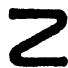
\includegraphics[keepaspectratio]{images/part002_f683a60c9eaa907b29b9c0e21fae4a1da7b4dd647e1d1a410962ae330fdaf4f4.jpg}}

Let F be a subset of an ordered set E, and let A be a subset of F. It can happen that one of the two elements \(\sup_{E} A\) , \(\sup_{F} A\) exists but the other does not, or that both exist but are unequal.

Examples

* (1) In the ordered set \(\mathbf{E} = \mathbf{R}\) of real numbers, consider the subset \(\mathbf{F} = \mathbf{Q}\) of rational numbers and the set \(\mathbf{A} \subset \mathbf{F}\) of rational numbers \(< \sqrt{2}\) ; \(\sup_{\mathbf{E}} \mathbf{A}\) exists but \(\sup_{\mathbf{F}} \mathbf{A}\) does not.

\begin{enumerate}
\def\labelenumi{(\arabic{enumi})}
\setcounter{enumi}{1}
\item
  In the notation of Example 1, let G be the union of A and the set \(\{2\}\) ; then \(G \subset F\) and \(\sup_{G} A\) exists, but \(\sup_{F} A\) does not.
\item
  With the same notation, \(\sup_{\mathbf{E}} \mathbf{A} = \sqrt{2}\) , \(\sup_{\mathbf{G}} \mathbf{A} = 2\) . *
\end{enumerate}

However, we have the following result :

PROPOSITION 9. Let E be an ordered set, F a subset of E, A a subset of F. If both \(\sup_{\mathbf{E}}\mathbf{A}\) and \(\sup_{\mathbf{F}}\mathbf{A}\) exist, we have \(\sup_{\mathbf{E}}\mathbf{A} \leqslant \sup_{\mathbf{F}}\mathbf{A}\) . If \(\sup_{\mathbf{E}}\mathbf{A}\) exists and belongs to F, then \(\sup_{\mathbf{F}}\mathbf{A}\) exists and is equal to \(\sup_{\mathbf{E}}\mathbf{A}\) .

The first assertion follows from the fact that the set M of upper bounds of A in F is contained in the set N of upper bounds of A in E, and from Proposition 5. On the other hand, if the least element of N lies in F, then it belongs to M and is clearly the least element of M; this proves the second assertion.

